\section{Amplificatore alle differenze}
\begin{wrapfigure}[14]{l}[0pt]{35mm}
	\caption{Schema dell'amplificatore alle differenze}
	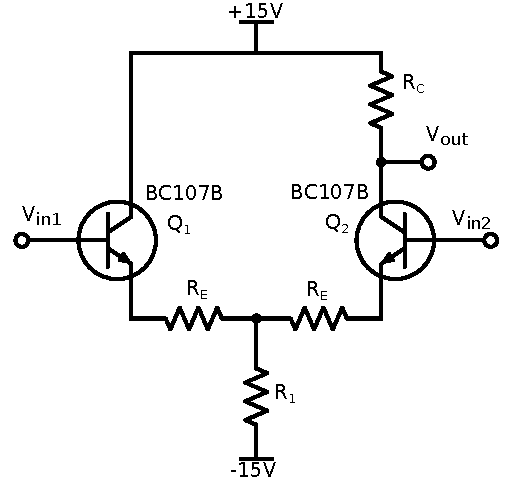
\includegraphics[width=35mm]{cc1.pdf}
	\label{fig:cc1}
\end{wrapfigure}

Un amplificatore alle differenze è un circuito che amplifica la differenza di due segnali in ingresso. 
Il circuito da noi realizzato è rappresentato in Fig. \ref{fig:cc1}.
L'obiettivo era quello di ottenere una corrente di quiescenza $I_q=\SI{0.5}{\milli\ampere}$, un guadagno differenziale $G_{diff}\approx 30$ e un guadagno a modo comune inferiore a $G_{CM} = 1$.
Abbiamo scelto di ultilizzare il valori delle resistenze fornitici dagli assistenti di laboratorio per semplicità.

Possiamo dunque imporre la seguente condizione:

\begin{equation}
V_B-V_E=2I_q R_1 + I_q R_E + 0.6
\label{eq:1}
\end{equation}

Tale equazione tiene conto della geometria del circuito.
Come vediamo, essa non permette tuttavia il calcolo diretto di $R_E$ ed $R_1$.
Per fare ciò è necessario imporre la condizione di $G_{diff} \approx 30$:

\begin{equation}
G_{diff}=\frac{R_C}{2(R_E+r_e)}
\label{eq:2}
\end{equation}

Con $r_e$ resistenza intrinseca dell'emettitore.
Come abbiamo appreso dallo studio del modello di $Early$, essa può essere stimata dall'equazione sperimentale $r_e = \left[ \frac{25}{I_q} \right] \Omega$.
Imponendo una corrente di quiescenza di \SI{0.5}{\milli\ampere} otteniamo immediatamente $r_e = 50\, \Omega$. 

Infine, avendo utilizzato una $R_C=(9.972\pm0.002),\si{\kilo\ohm}$, è possibile attraverso eq. (\ref{eq:1}) e eq. (\ref{eq:2}) stimare i valori adeguati di $R_1$ ed $R_E$. 

Come consigliato in laboratorio, sono state utilizzate una $R_E=(118.9\pm0.5) \,\Omega$\footnote{In questo caso abbiamo scelto di eseguire un valor medio dei due valori misurati con il multimetro e di stimare un errore massimo definito come la semi-differenza dei due valori. Così facendo anche invertendo le resistenze nel circuito il valore reale sarà sempre compatibile con quello assunto nei calcoli.} e una $R_1= (9.933 \pm 0.002)\,\si{\kilo\ohm}$.
Con questi valori di resistenza la corrente di quiescenza $I_q$ è di \SI{0.7}{\milli\ampere} (sperimentalmente abbiamo misurato una corrente di $(0.719 \pm 0.003) \si{\milli\ampere}$.

Per rendere l'analisi dei segnali più semplice, abbiamo collegato il $V_{in}2$ a terra.
Così facendo abbiamo ottenuto solo un'amplificazione del segnale in ingresso a $V_{in}1$. 

Riportiamo ora (in Fig. \ref{fig:sig}) un grafico dei dati sperimentali acquisiti. 

\begin{figure}[h]
\centering
	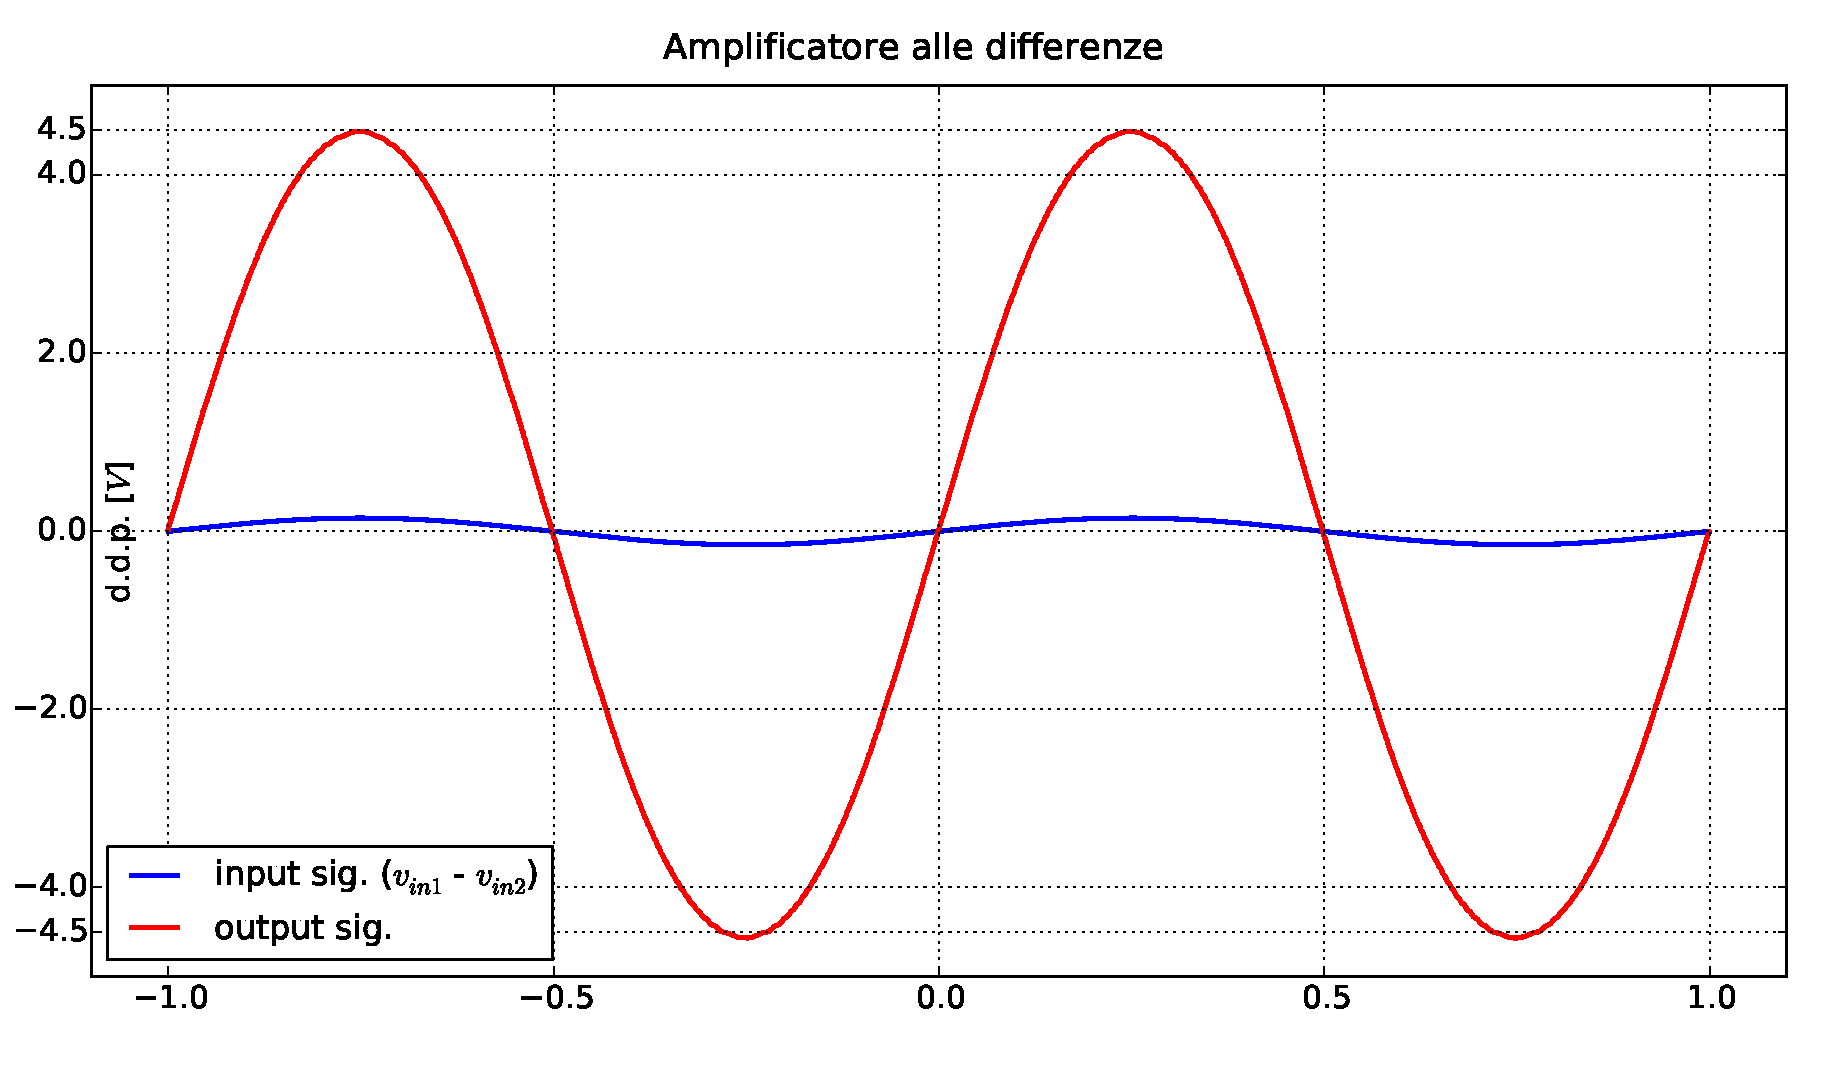
\includegraphics[scale=0.425]{accontentati.pdf}
	\caption{.}
	\label{fig:sig}
\end{figure}

Il guadagno è stato stimato dai valori picco-picco del segnale in ingresso e di quello in input:

$$G_{diff}=\frac{V_{out}}{V_{in}}$$

Sperimentalmente abbiamo ottenuto il valore $G_{diff}=30.1 \pm 0.1$


Utilizzando eq. (\ref{eq:2}) è possibile calcolare il valore di resistenza intrinseca dell'emettitore: $r_e=\frac{R_c-2R_E G_{diff}}{2G_{diff}}$.
Sfruttando la composizione degli errori, abbiamo ottenuto il valore $r_e=(46.7\pm0.8)\,\Omega$.

Abbiamo dunque calcolato il guadagno in modo comune definito come :

\begin{equation}
G_{CM}=-\frac{R_C}{2R_1+R_E+	r_e}
\label{eq:3}
\end{equation}

Ricordiamo che il segno meno indica uno sfasamento tra i segnali di $\pi$.
Sperimentalmente tale guadagno può essere calcolato ponendo $V_{in1}=V_{in2}$ e facendo il rapporto (nel nostro caso picco-picco) tra segnale in ingresso e in uscita:

$$G_{CM}=\frac{V_{out}}{V_{in}}$$

Il valore sperimentale risulta essere $G_{CM} = -0.483 \pm 0.003$. Anche in questo caso abbiamo provato a calcolare il valore di $r_e$ partendo da eq.(\ref{eq:3}) ma senza successo.
Infatti non risulta possibile stimare in modo preciso il valore di resistenza intrinseca dell'emettitore partendo da tale equazione in quanto esso è proporzionale all'inverso di $G_{CM}$ il quale è un valore inferiore a 1.
Piccole variazioni nel guadagno in modo comune causano enormi cambiamenti nel valore di $r_e$. 

Infine abbiamo calcolato il fattore di reiezione a modo comune (Common Mode Reaction Ratio):

\begin{equation}
CMRR=\frac{G_{diff}}{G_{CM}}=62.3\pm0.5
\end{equation}

Più tale fattore risulta alto e più l'amplificatore alle differenze è efficace. Se ad esempio abbiamo un rumore identico su entrambi i canali di ingresso, un CMRR alto garantisce una riduzione di tale rumore sul segnale in output.

\section{Amplificatore alle differenze con sorgente di corrente}
\begin{wrapfigure}[16]{l}[0pt]{35mm}
	\caption{.}
	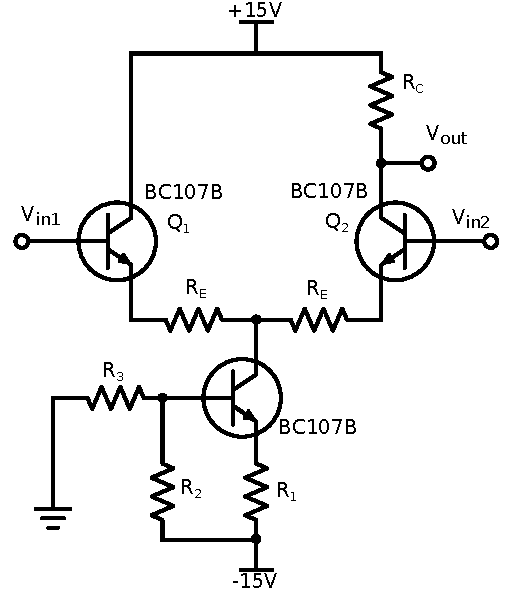
\includegraphics[width=35mm]{cc2.pdf}
	\label{fig:cc2}
\end{wrapfigure}


Per migliorare il valore di $G_{CM}$ e di conseguenza quello di $CMRR$, si posiziona una sorgente di corrente costante a valle del circuito, come mostrato in Fig. \ref{fig:cc2}.

In questa seconda parte dell'esperienza abbiamo analizzato il comportamento del circuito modificato con la sorgente di corrente costante.
Al circuito sono state aggiunte due resistenze di valore $R_2 = (1507.5 \pm 0.5)\,\si{\ohm}$ e $R_3 = (32.723 \pm 0.003)\,\si{\kilo\ohm}$ e un ulteriore transistor BC107B.

Come fatto per il circuito precedente, abbiamo ricavato i valori del guadagno differenziale, del guadagno in modo comune e del fattore di reiezione a modo comune.

\begin{equation}
	G_{diff} = \frac{V_{out}}{V_{in}} _{V_{in1} \neq V_{in2}} = 32.05 \pm ??
\end{equation}
\begin{equation}
	G_{CM} = \frac{V_{out}}{V_{in}} _{V_{in1} = V_{in2}} = ?? \pm ??
\end{equation}
\begin{equation}
	CMRR = \frac{G_{CM}}{G_{diff}} = ?? \pm ??
\end{equation}